\chapter{Coloring}
Rishnak  was impressed with Ajur's logical reasoning ability and went looking for him. He found Ajur ambling along with Jura and caught up with them. (Ghosts can move rather quickly.) Rishnak asked Ajur if he likes coloring.  Ajur enthusiastically responded that he did indeed like to color and enjoyed its calming effect.

Rishnak was pleased with this response and introduced the next topic: graph colorings. A proper \emph{vertex coloring} of a graph is a coloring of vertices such that no adjacent vertices (i.e., vertices connected by an edge) have the same color. An interesting problem is to determine the smallest number of colors to properly vertex color a graph. 
Then Rishnak showed an example of proper coloring of a graph in Figure \ref{10g1} with 4 colors. Ajur jumped up and down and said that he could color it with three colors and showed his coloring in Figure \ref{10g2}.
\begin{figure}[h]
\begin{center}
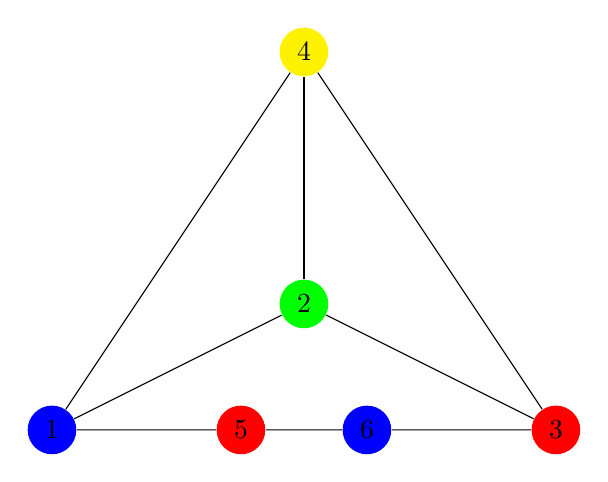
\begin{tikzpicture}
  [scale=.8,auto=left,every node/.style={circle}]
  \node (n1)[fill=blue] at (-1,7) {1};
  \node (n2)[fill=green] at (3,9)  {2};
  \node (n3)[fill=red] at (7,7)  {3};
  \node (n4)[fill=yellow] at (3,13)  {4};
  \node (n5)[fill=red] at (2,7) {5};
  \node (n6)[fill=blue] at (4,7) {6};
 \foreach \from/\to in {n1/n2,n2/n3,n2/n4,n1/n4,n3/n4,n1/n5,n5/n6,n6/n3}
    \draw (\from) -- (\to);
\end{tikzpicture}
\caption{ Proper Coloring the vertices of a graph with 4 colors}\label{10g1}
\end{center}
\end{figure}

\begin{figure}[h]
\begin{center}
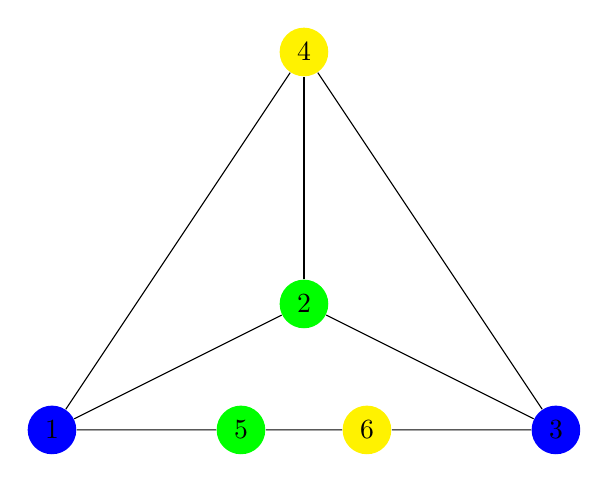
\begin{tikzpicture}
  [scale=.8,auto=left,every node/.style={circle}]
  \node (n1)[fill=blue] at (-1,7) {1};
  \node (n2)[fill=green] at (3,9)  {2};
  \node (n3)[fill=blue] at (7,7)  {3};
  \node (n4)[fill=yellow] at (3,13)  {4};
  \node (n5)[fill=green] at (2,7) {5};
  \node (n6)[fill=yellow] at (4,7) {6};
 \foreach \from/\to in {n1/n2,n2/n3,n2/n4,n1/n4,n3/n4,n1/n5,n5/n6,n6/n3}
    \draw (\from) -- (\to);
\end{tikzpicture}
\caption{ Proper Coloring the vertices of a graph with 3 colors}\label{10g2}
\end{center}
\end{figure}

Ajur added that 3 colors are needed as vertices 1, 2 and 4 are mutually adjacent and those vertices need 3 different colors. 
Rishnak asked Ajur to properly color the graph $K_{3,3}$, a complete bipartite graph. Ajur jumped at the opportunity and showed a 2 coloring of this graph \ref{10g3}
\begin{figure}
\begin{center}
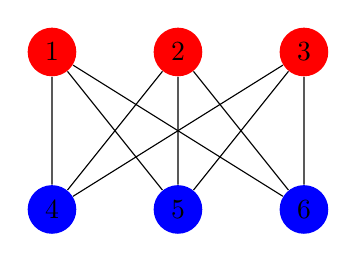
\begin{tikzpicture}
  [scale=.4,auto=left,every node/.style={circle}]
  \node (n1)[fill=red] at (1,7) {1};
  \node (n2)[fill=red] at (5,7)  {2};
  \node (n3)[fill=red] at (9,7) {3};
  \node (n4) [fill=blue] at (1,2)  {4};
  \node (n5) [fill=blue] at (5,2) {5};
  \node (n6)[fill=blue] at (9,2)  {6};
 
  
   \foreach \from/\to in {n1/n6,n1/n4,n1/n5,n2/n6,n2/n4,n2/n5,n3/n4,n3/n5,n3/n6}
    \draw (\from) -- (\to);
    \end{tikzpicture}
\caption{ Two coloring of a Bipartite Graph with 6 vertices and 9 edges, denoted by $K_{3,3}$}\label{10g3}
\end{center}
\end{figure}

Ajur explained: in a bipartite graph the vertices are partitioned into two sets $A$ and $B$ and the edges always go from $A$ to $B$. Ajur further stated that all the vertices in $A$ can be colored with one color, say red, and all the vertices in $B$ can be colored with another color, say blue. Since all trees are also bipartite graphs, trees can be colored with just two colors, exactly as in Figure \ref{10g4}. Coloring trees reminded Ajur of the beautiful fall colors one sees in the trees!
\begin{figure}
\begin{center}

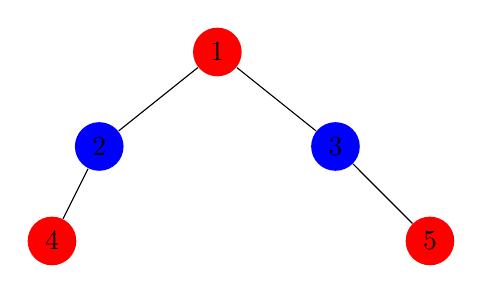
\begin{tikzpicture}
  [scale=.6,auto=left,every node/.style={circle}]
  \node (n1)[fill=red] at (5.5,7) {1};
  \node (n2)[fill=blue] at (3,5)  {2};
  \node (n3)[fill=blue] at (8,5)  {3};
  \node (n4)[fill=red] at (2,3) {4};
  \node (n5)[fill=red] at (10,3)  {5};


  \foreach \from/\to in {n1/n2,n1/n3,n2/n4,n3/n5}
    \draw (\from) -- (\to);

\end{tikzpicture}

\caption{Two coloring of a tree }\label{10g4}
\end{center}
\end{figure}

Ajur was getting curious and asked "can one color edges too? How are adjacent edges defined?"  Rishnak always believed that asking the right questions is important because it is a signal that one's understanding is deepening. Rishnak responded: two edges are adjacent if they are incident to the same vertex. For example consider the graph shown in Figure \ref{10g5},
edge $e_1$ is adjacent to $e_2$ (both are incident at vertex 1) and to $e_3$, $e_4$ and $e_5$ as all these edges are incident at vertex 2. A four edge coloring of this graph is shown in Figure \ref{10g5}. 

\begin{figure}
\begin{center}

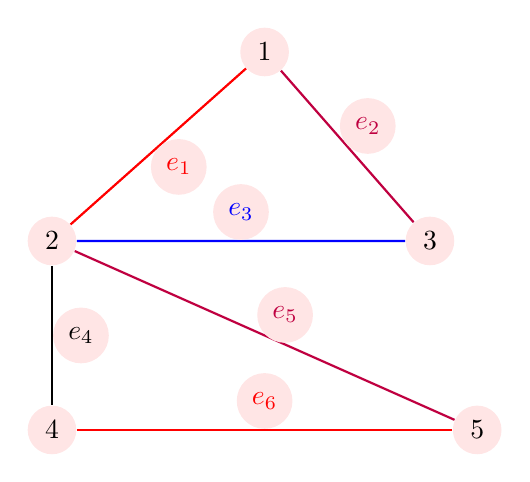
\begin{tikzpicture}
  [scale=.6,auto=left,every node/.style={circle,fill=red!10}]
  \node (n1) at (5.5,9) {1};
  \node (n2) at (1,5)  {2};
  \node (n3) at (9,5)  {3};
  \node (n4) at (1,1) {4};
  \node (n5) at (10,1)  {5};

\path[-,draw,thick]
    (n1) edge [color=red] node {$e_1$} (n2)
    (n1) edge [color=purple] node {$e_2$} (n3)
    (n2) edge [color=blue] node {$e_3$} (n3)
    (n2) edge [color=black] node {$e_4$} (n4)
    (n2) edge [color=purple] node {$e_5$}  (n5)
    (n4) edge [color=red]node {$e_6$}  (n5)
    ;

\end{tikzpicture}

\caption{Four Edge Coloring of a Graph, edge $e_1$ is adjacent to $e_2$, $e_3$,
$e_4$ and $e_5$}\label{10g5}
\end{center}
\end{figure}

Ajur exclaimed that the maximum degree in this graph is 4 and that is why it needs 4 colors and 4 colors seem to be sufficient. Rishnak smiled and said Ajur's observation relating to maximum degree of a graph is good. However, the maximum degree of graph being $\Delta$ does not imply that the graph has a $\Delta$-coloring. Rishnak explained that in a cycle of length 5, the maximum degree is 2 but it needs 3 colors to color its edges.

\begin{figure}
\begin{center}

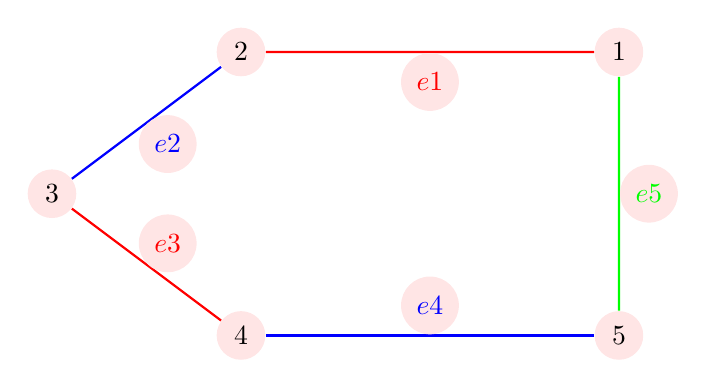
\begin{tikzpicture}
  [scale=.6,auto=left,every node/.style={circle, fill=red!10}]
  \node (n1) at (10,9) {1};
  \node (n2) at (2,9)  {2};
  \node (n3) at (-2,6)  {3};
  \node (n4) at (2,3) {4};
  \node (n5) at (10,3)  {5};

\path[-,draw,thick]
    (n1) edge [color=red] node {$e1$} (n2)
    (n2) edge [color=blue] node {$e2$} (n3)
    (n3) edge [color=red] node {$e3$} (n4)
    (n4) edge [color=blue] node {$e4$} (n5)
    (n1) edge [color=green] node {$e5$}  (n5)
;
\end{tikzpicture}

\caption{Three edge coloring of a cycle of length 5 }\label{10g6}
\end{center}
\end{figure}

Rishnak told Ajur that a graph with maximum degree $\Delta$ can be edge colored with either $\Delta$ or $\Delta+1$ colors. A regular graph with degree three that needs four edge colors for a proper edge coloring is known as a \emph{Snark}. Ajur had heard of Snarks from a poem by his dad's favorite author Lewis Carroll
\textbf{The Hunting of the Snarks}. Rishnak smiled and said that graph theorists have a whimsical sense of humor and since four-edge-colorable trivalent graphs are elusive, they named these graphs Snarks.
Ajur became curious to find one himself and asked if the Petersen graph is a snark. Surprised that Ajur remembered, Rishank replied that the Petersen graph, a regular graph of degree 3, indeed needs 4 colors to color the edges of that graph, see Figure \ref{10g7}
\begin{figure}
\begin{center}
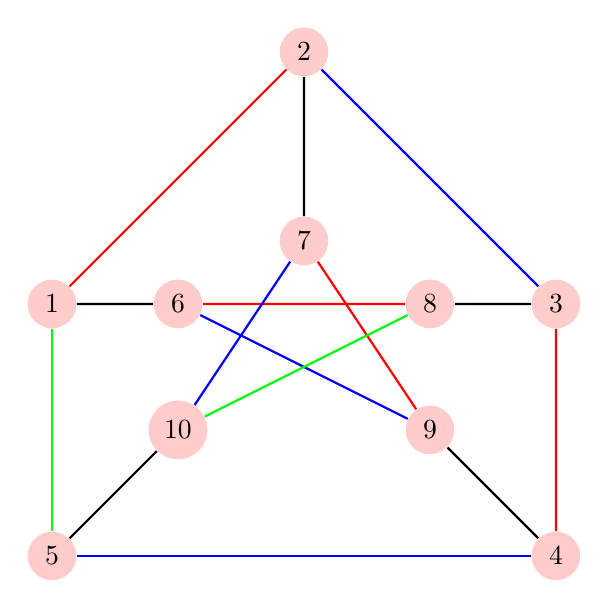
\begin{tikzpicture}
  [scale=.8,auto=left,every node/.style={circle,fill=red!20}]
  \node (n1) at (1,7) {1};
  \node (n2) at (5,11)  {2};
  \node (n3) at (9,7)  {3};
  \node (n4) at (9,3) {4};
  \node (n5) at (1,3) {5};
  \node (n6) at (3,7)  {6};
  \node (n7) at (5,8) {7};
  \node (n8)  at (7,7) {8};
  \node (n9) at (7,5) {9};
  \node (n10) at  (3,5) {10};
 \path[-,draw,thick]
    (n1) edge [color=red]  (n2)
    (n2) edge [color=blue]   (n3)
    (n3) edge [color=red]  (n4)
    (n4) edge [color=blue]  (n5)
    (n1) edge [color=green]  (n5)
    (n7) edge [color=red]   (n9)
    (n9) edge [color=blue]   (n6)
    (n6) edge [color=red]  (n8)
    (n8) edge [color=green]   (n10)
    (n10) edge [color=blue]  (n7)
    (n1) edge [color=black] (n6)
    (n2) edge [color=black] (n7)
    (n3) edge [color=black] (n8)
    (n4) edge [color=black] (n9)
    (n5) edge [color=black] (n10)
    ;

\end{tikzpicture}
\caption{ 4 edge coloring of Petersen Graph,a regular graph of degree 3, a snark }\label{10g7}
\end{center}
\end{figure}

One can convert an edge coloring problem to a vertex coloring problem. From a graph , $G$, where you want to color the edges, construct a new graph, $H$, in which edges of the original graph $G$ become vertices of the new graph $H$ and two vertices in $H$ are adjacent if the corresponding edges in $G$ are incident on the same vertex of $G$.
For example, an edge coloring of \ref{10g4} can be converted into a vertex coloring of \ref{10g45}.
\begin{figure}
\begin{center}

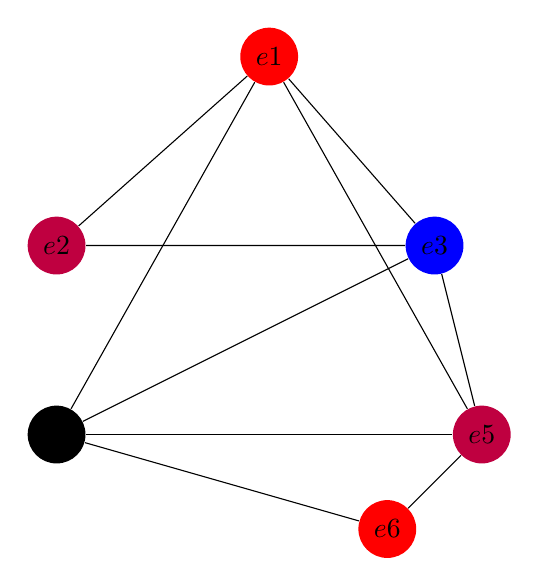
\begin{tikzpicture}
  [scale=.6,auto=left,every node/.style={circle}]
  \node (n1)[fill=red] at (5.5,9) {$e1$};
  \node (n2)[fill=purple] at (1,5)  {$e2$};
  \node (n3)[fill=blue] at (9,5)  {$e3$};
  \node (n4)[fill=black] at (1,1) {$e4$};
  \node (n5)[fill=purple] at (10,1)  {$e5$};
  \node (n6)[fill=red] at (8,-1) {$e6$};

 \foreach \from/\to in {n1/n2,n1/n3,n1/n5,n1/n4,n2/n3,n3/n5,n3/n4,n4/n5,n4/n6,n5/n6}
    \draw (\from) -- (\to);

\end{tikzpicture}

\caption{Four vertex Coloring of a Graph, corresponding to the 4 edge coloring of Graph \ref{10g5}}\label{10g45}
\end{center}
\end{figure}


Rishnak then talked about an interesting puzzle, somewhat related to the edge coloring problem. In a group of 6 people, say Alexis, Baily, Charles, Danny, Elaine and Frances, every pair could be friends or enemies. For example, Charles is friends with Alexis and Baily and Charles and the other three are enemies. Rishnak asked Ajur to prove that in a group of 6 people, there will be at least three people who are mutually friends to each other or who are mutually enemies to each other. Ajur said that he could model this problem as a complete graph on 6 vertices. Color the 15 edges either red or blue. Color red denotes they are enemies and blue means they are friends. Ajur rephrased Rishank's question as no matter how you color the edges, there will always be a red triangle or a blue triangle. Rishnak was impressed with Ajur's ability to translate the given problem into a graph theoretic problem even if he could not solve it.\footnote{Please work out the full solution}


The map coloring problem is to color the regions or faces of a \emph{planar} graph (maps are usually drawn on a plane) so that no two adjacent faces or regions are colored the same. Here is an example of a map coloring
of the graph in Figure \ref{10g8}. The four faces are (1,2,4,6), (1,3,4,5), (2,3,5,6) and (4,5,6). Each of these regions share a border (or an edge) with other region. Hence all these four regions are mutually adjacent. Often the outside region is also colored. In Figure \ref{10g8} the outside region could be colored with yellow (as it does share a border with the region (4,5,6). and we still need four colors.
\begin{figure}
\begin{center}
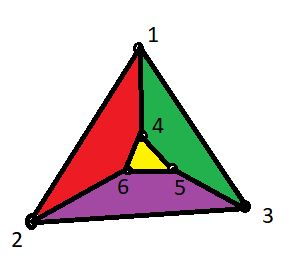
\includegraphics[width=0.5\textwidth]{mapcolor.JPG}
\end{center}
\caption{A graph with 4 regions or faces and each region or face is colored differently}\label{10g8}
\end{figure}

One of the most famous theorems about map coloring states that every planar graph can be map colored with 4 colors. That is, we need only 4 colors to color every region so that no two adjacent regions are colored the same. Here is an example of the map of USA colored with 4 colors. Of course, the region or face in this map are the states of USA. It is not like the normal USA map you see in an atlas; the states are not to-scale. But this map of USA preserves the adjacency relationships. Rishnak asked Ajur can you spot the state of Maine in this Figure \ref{10g9}
\begin{figure}
\begin{center}
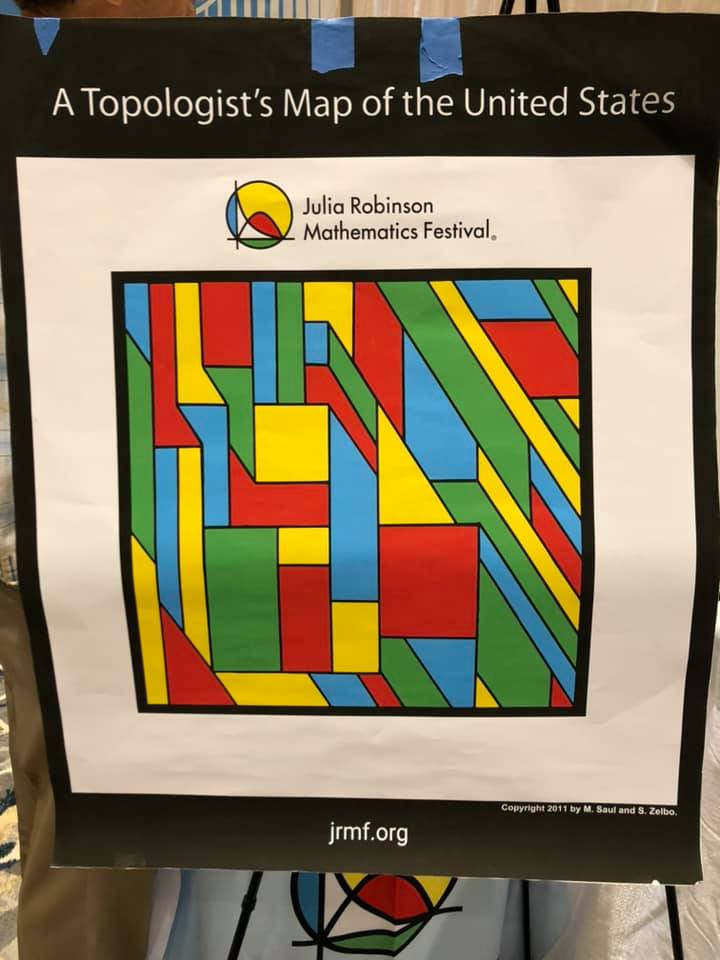
\includegraphics[width=0.5\textwidth]{usamap.png}
\end{center}
\caption{USA Map with faces/states adjacency preserved}\label{10g9}
\end{figure}

Ajur thought for a while. Ajur knew that the state of Maine borders with only one adjacent state that of New Hampshire. So he immediately replied that the region colored yellow in the north east corner is the state of Maine.

Rishnak showed Ajur the map of India with state names given in Figure \ref{10g10}. Rishnak asked Ajur whether the state of Andhra Pradesh and Kerala could be colored the same color?

\begin{figure}
\begin{center}
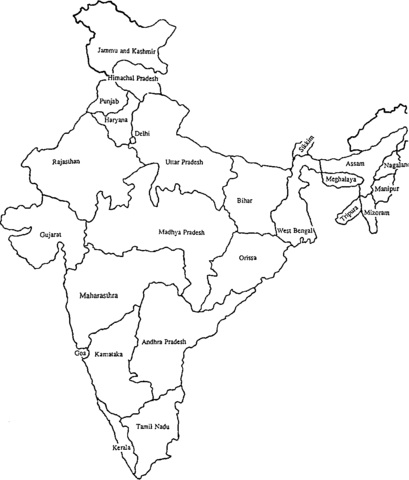
\includegraphics[width=0.9\textwidth]{MapIndia.jpg}
\end{center}
\caption{India Map with faces/states adjacency preserved}\label{10g10}
\end{figure}

Ajur had no hesitation in saying that they could be colored the same color as they share no boundaries or edges. Rishnak asked how about whether Goa and Kerala can be colored the same color. Ajur replied instantaneously with a resounding yes. Ajur asked Rishnak whether the map coloring problem can be converted to a vertex coloring (similar to conversion of edge coloring problem to vertex coloring problem). Ajur further explained that each region/face of the original map would have to become a vertex of the new graph and two vertices in the new graph are adjacent if the corresponding faces in the old graph will share an edge. For example in the continental US map, all the states (faces of the original graph) will become vertices of the new graph and two vertices are adjacent, if the corresponding states share a border in the original graph. For example the vertex corresponding to Maine will be just adjacent to the vertex corresponding to the state of New Hampshire. Similarly, the vertex corresponding to the state of Washington will be adjacent to the vertices corresponding to Oregon and Idaho. Rishnak was very pleased with the way Ajur was absorbing the material. Rishnak did not want to push further and called it a day. Ajur and Jura were very happy to be left alone. 